\documentclass{article}\usepackage[]{graphicx}\usepackage[]{color}
% maxwidth is the original width if it is less than linewidth
% otherwise use linewidth (to make sure the graphics do not exceed the margin)
\makeatletter
\def\maxwidth{ %
  \ifdim\Gin@nat@width>\linewidth
    \linewidth
  \else
    \Gin@nat@width
  \fi
}
\makeatother

\definecolor{fgcolor}{rgb}{0.345, 0.345, 0.345}
\newcommand{\hlnum}[1]{\textcolor[rgb]{0.686,0.059,0.569}{#1}}%
\newcommand{\hlstr}[1]{\textcolor[rgb]{0.192,0.494,0.8}{#1}}%
\newcommand{\hlcom}[1]{\textcolor[rgb]{0.678,0.584,0.686}{\textit{#1}}}%
\newcommand{\hlopt}[1]{\textcolor[rgb]{0,0,0}{#1}}%
\newcommand{\hlstd}[1]{\textcolor[rgb]{0.345,0.345,0.345}{#1}}%
\newcommand{\hlkwa}[1]{\textcolor[rgb]{0.161,0.373,0.58}{\textbf{#1}}}%
\newcommand{\hlkwb}[1]{\textcolor[rgb]{0.69,0.353,0.396}{#1}}%
\newcommand{\hlkwc}[1]{\textcolor[rgb]{0.333,0.667,0.333}{#1}}%
\newcommand{\hlkwd}[1]{\textcolor[rgb]{0.737,0.353,0.396}{\textbf{#1}}}%
\let\hlipl\hlkwb

\usepackage{framed}
\makeatletter
\newenvironment{kframe}{%
 \def\at@end@of@kframe{}%
 \ifinner\ifhmode%
  \def\at@end@of@kframe{\end{minipage}}%
  \begin{minipage}{\columnwidth}%
 \fi\fi%
 \def\FrameCommand##1{\hskip\@totalleftmargin \hskip-\fboxsep
 \colorbox{shadecolor}{##1}\hskip-\fboxsep
     % There is no \\@totalrightmargin, so:
     \hskip-\linewidth \hskip-\@totalleftmargin \hskip\columnwidth}%
 \MakeFramed {\advance\hsize-\width
   \@totalleftmargin\z@ \linewidth\hsize
   \@setminipage}}%
 {\par\unskip\endMakeFramed%
 \at@end@of@kframe}
\makeatother

\definecolor{shadecolor}{rgb}{.97, .97, .97}
\definecolor{messagecolor}{rgb}{0, 0, 0}
\definecolor{warningcolor}{rgb}{1, 0, 1}
\definecolor{errorcolor}{rgb}{1, 0, 0}
\newenvironment{knitrout}{}{} % an empty environment to be redefined in TeX

\usepackage{alltt}

\usepackage{float}

% Set the margins on the page to not be so large
\addtolength{\oddsidemargin}{-.875in}
\addtolength{\evensidemargin}{-.875in}
\addtolength{\textwidth}{1.75in}
\addtolength{\topmargin}{-.875in}
\addtolength{\textheight}{1.75in}

% Take off page numbering
\pagenumbering{gobble}
\IfFileExists{upquote.sty}{\usepackage{upquote}}{}
\begin{document}

\title{%
  3.2.1 - R: Variable Selection \\
  \smallskip
  \large Stat 5100: Dr. Bean
}
\date{}

\maketitle

\textbf{Example:} (Textbook tables 9.1 \& 9.5)  A hospital surgical unit was interested in predicting survival time for patients who undergo a particular liver operation.  Data are reported for 108 patients on the following variables:  blood-clotting score, prognostic index, enzyme function test score, liver function test score, age (in years), gender (0=male, 1=female), indicators of alcohol use (none, moderate, heavy), and survival time (in days).  Which (if any) of these predictors should be used in a linear model?

\subsubsection*{Create train/test data and check assumptions}

\begin{knitrout}
\definecolor{shadecolor}{rgb}{0.969, 0.969, 0.969}\color{fgcolor}\begin{kframe}
\begin{alltt}
\hlcom{# Set a random seed so that results are reproducible}
\hlkwd{set.seed}\hlstd{(}\hlnum{2341}\hlstd{)}

\hlcom{# Load the data}
\hlkwd{library}\hlstd{(stat5100)}
\hlkwd{data}\hlstd{(surgical)}

\hlcom{# We commonly will make our test set be 1/3 of the data, and have our training}
\hlcom{# set be the other 2/3 of the data. There are a variety of ways to randomly}
\hlcom{# split up the data this way, here is one efficient way to do it:}
\hlstd{n} \hlkwb{<-} \hlkwd{nrow}\hlstd{(surgical)}
\hlstd{train_index} \hlkwb{<-} \hlkwd{sample}\hlstd{(}\hlnum{1}\hlopt{:}\hlstd{n,} \hlkwc{size} \hlstd{= (}\hlnum{2}\hlopt{/}\hlnum{3}\hlstd{)}\hlopt{*}\hlstd{n)}
\hlstd{train_surgical} \hlkwb{<-} \hlstd{surgical[train_index, ]}
\hlstd{test_surgical} \hlkwb{<-} \hlstd{surgical[}\hlopt{-}\hlstd{train_index, ]}

\hlcom{# Check initial assumptions using the training data}
\hlstd{surgical_train_lm} \hlkwb{<-} \hlkwd{lm}\hlstd{(Time} \hlopt{~} \hlstd{bloodclot} \hlopt{+} \hlstd{prognostic} \hlopt{+} \hlstd{enzyme} \hlopt{+} \hlstd{liver,}
                        \hlkwc{data} \hlstd{= train_surgical)}
\hlstd{stat5100}\hlopt{::}\hlkwd{visual_assumptions}\hlstd{(surgical_train_lm)}
\end{alltt}
\end{kframe}

{\centering 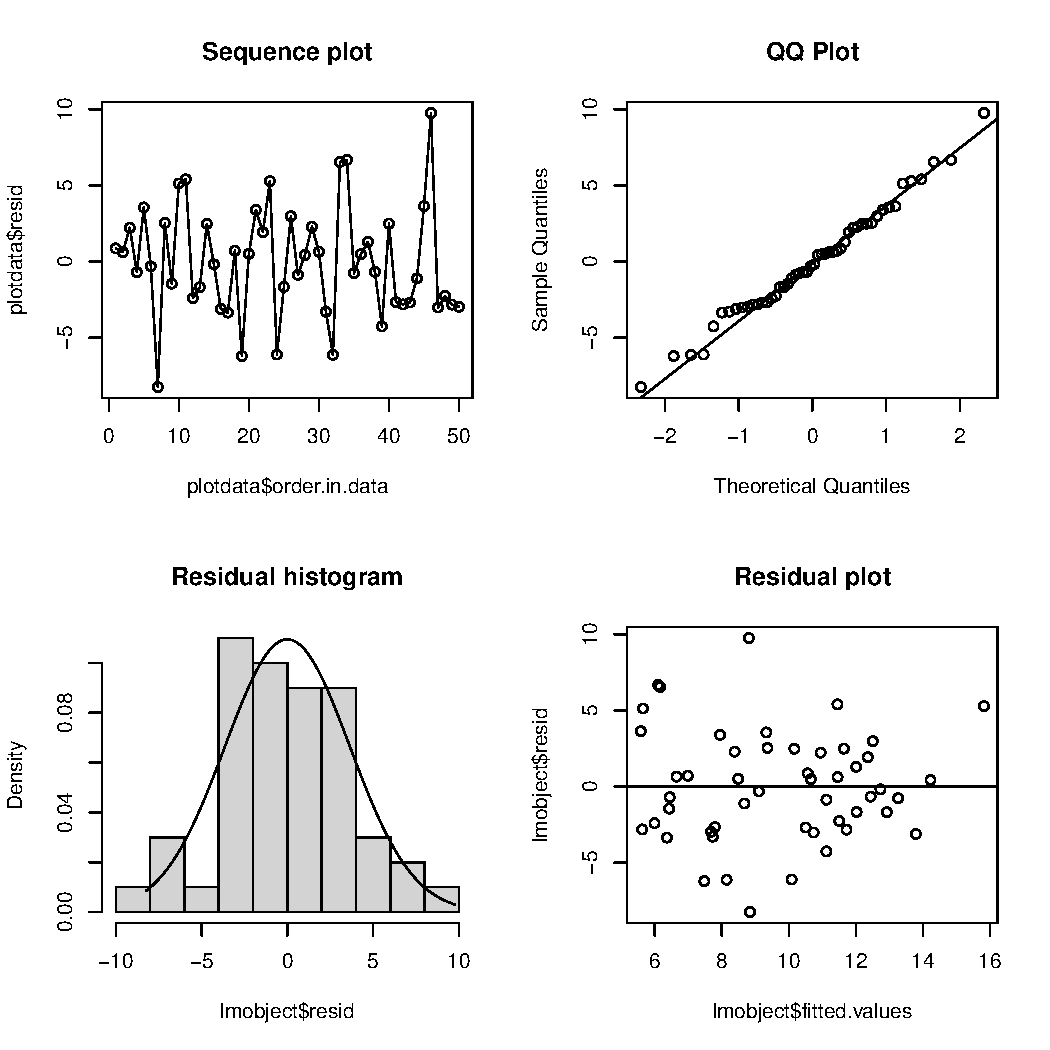
\includegraphics[width=0.6\textwidth]{figure/unnamed-chunk-1-1} 

}


\begin{kframe}\begin{alltt}
\hlstd{stat5100}\hlopt{::}\hlkwd{brown_forsythe_lm}\hlstd{(surgical_train_lm)}
\end{alltt}
\begin{verbatim}
## [1] "Brown-forsythe test for constant variance in the residuals:"
## [1] "T-statistic: -0.8723, p-value: 0.386"
\end{verbatim}
\begin{alltt}
\hlstd{stat5100}\hlopt{::}\hlkwd{cor_normality_lm}\hlstd{(surgical_train_lm)}
\end{alltt}
\begin{verbatim}
## Correlation test of normality:
##                   resid expected_norm
## resid         1.0000000     0.9868459
## expected_norm 0.9868459     1.0000000
## 
## Total observations: 72
## Make sure to consult with table B.6 for your final result.
\end{verbatim}
\end{kframe}
\end{knitrout}

\subsubsection*{Consider a possible transformation on the response}

\begin{knitrout}
\definecolor{shadecolor}{rgb}{0.969, 0.969, 0.969}\color{fgcolor}\begin{kframe}
\begin{alltt}
\hlstd{MASS}\hlopt{::}\hlkwd{boxcox}\hlstd{(surgical_train_lm)}
\end{alltt}
\end{kframe}

{\centering 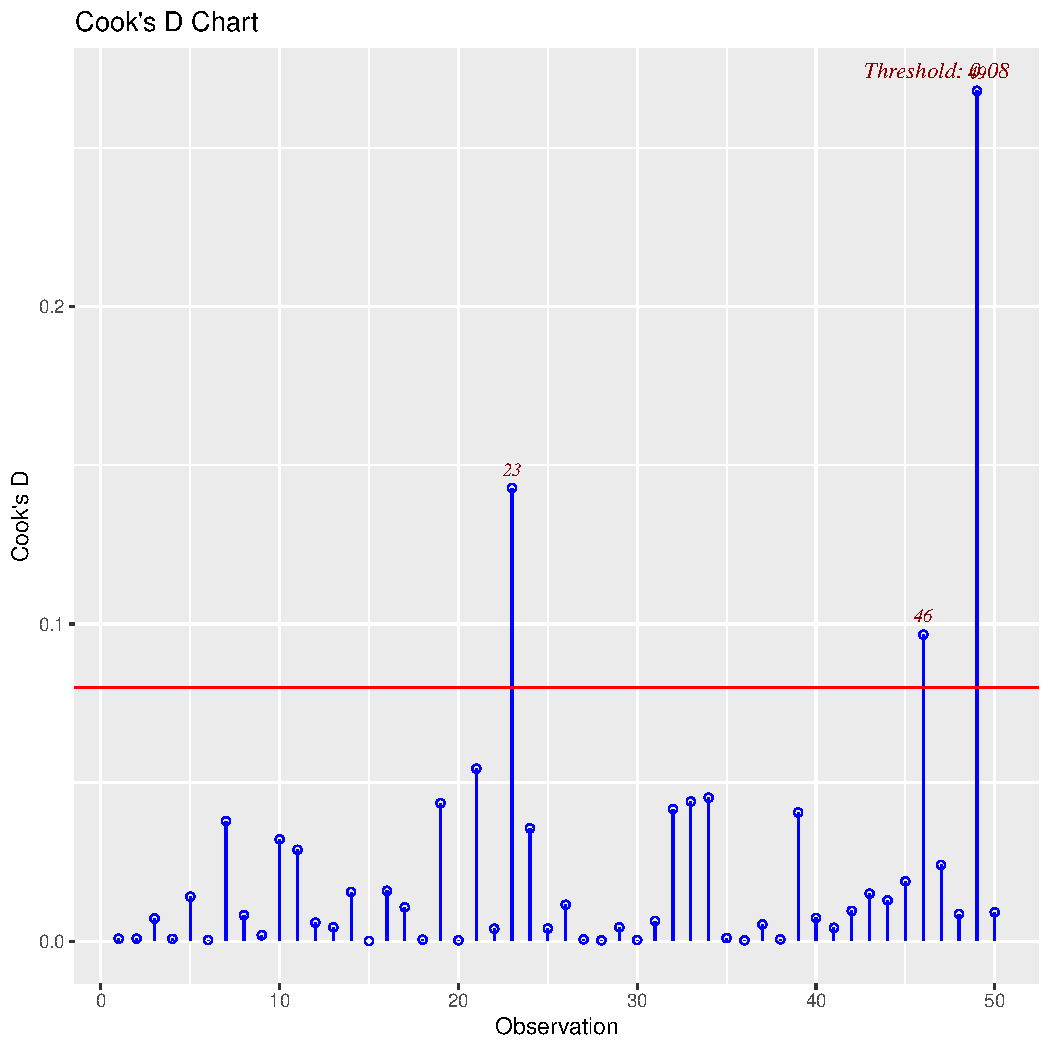
\includegraphics[width=0.6\textwidth]{figure/unnamed-chunk-2-1} 

}


\begin{kframe}\begin{alltt}
\hlcom{# Make a log-transform (Make sure to transform on both training and testing data)}
\hlstd{train_surgical} \hlkwb{<-} \hlkwd{cbind}\hlstd{(train_surgical,} \hlkwc{logTime} \hlstd{=} \hlkwd{log}\hlstd{(train_surgical}\hlopt{$}\hlstd{Time))}
\hlstd{test_surgical} \hlkwb{<-} \hlkwd{cbind}\hlstd{(test_surgical,} \hlkwc{logTime} \hlstd{=} \hlkwd{log}\hlstd{(test_surgical}\hlopt{$}\hlstd{Time))}

\hlcom{# Fit a new log model}
\hlstd{surgical_logtrain_lm} \hlkwb{<-} \hlkwd{lm}\hlstd{(logTime} \hlopt{~} \hlstd{bloodclot} \hlopt{+} \hlstd{prognostic} \hlopt{+} \hlstd{enzyme} \hlopt{+} \hlstd{liver,}
                           \hlkwc{data} \hlstd{= train_surgical)}
\end{alltt}
\end{kframe}
\end{knitrout}

\subsubsection*{Perform variable selection with $R^2$, adjusted $R^2$, or Mallow's $C_p$:}

Note that the output below shows results for \textit{all} possible combinations of variables in the model.

\begin{knitrout}
\definecolor{shadecolor}{rgb}{0.969, 0.969, 0.969}\color{fgcolor}\begin{kframe}
\begin{alltt}
\hlstd{olsrr}\hlopt{::}\hlkwd{ols_step_all_possible}\hlstd{(surgical_logtrain_lm)}
\end{alltt}
\begin{verbatim}
##    Index N                        Predictors   R-Square Adj. R-Square
## 3      1 1                            enzyme 0.40896416   0.400520790
## 4      2 1                             liver 0.36064018   0.351506464
## 2      3 1                        prognostic 0.28135339   0.271087005
## 1      4 1                         bloodclot 0.00904029  -0.005116277
## 8      5 2                 prognostic enzyme 0.69553296   0.686707831
## 10     6 2                      enzyme liver 0.51490091   0.500840063
## 9      7 2                  prognostic liver 0.47040155   0.455050871
## 6      8 2                  bloodclot enzyme 0.45254253   0.436674193
## 7      9 2                   bloodclot liver 0.36400730   0.345572731
## 5     10 2              bloodclot prognostic 0.28847685   0.267852989
## 11    11 3       bloodclot prognostic enzyme 0.73495360   0.723260372
## 14    12 3           prognostic enzyme liver 0.70644450   0.693493521
## 13    13 3            bloodclot enzyme liver 0.52249652   0.501430188
## 12    14 3        bloodclot prognostic liver 0.47137051   0.448048616
## 15    15 4 bloodclot prognostic enzyme liver 0.73540593   0.719609269
##    Mallow's Cp
## 3    81.660955
## 4    93.897461
## 2   113.974309
## 1   182.928906
## 8    11.096556
## 10   56.835857
## 9    68.103897
## 6    72.626125
## 7    95.044844
## 5   114.170520
## 11    3.114539
## 14   10.333558
## 13   56.912510
## 12   69.858541
## 15    5.000000
\end{verbatim}
\end{kframe}
\end{knitrout}

\subsubsection*{Perform variable selection with}

Note that the output below shows results for only a few different model choices. This function from the ``olsrr'' package will show more information criteria (including SBC, AIC, and more that we don't talk about in our class) but it will not show every single possible variable combination like the last section. On the second table, each of the result rows refers to a specific model number, which you can reference with the first table in the output.

\begin{knitrout}
\definecolor{shadecolor}{rgb}{0.969, 0.969, 0.969}\color{fgcolor}\begin{kframe}
\begin{alltt}
\hlstd{olsrr}\hlopt{::}\hlkwd{ols_step_best_subset}\hlstd{(surgical_logtrain_lm)}
\end{alltt}
\begin{verbatim}
##             Best Subsets Regression             
## ------------------------------------------------
## Model Index    Predictors
## ------------------------------------------------
##      1         enzyme                            
##      2         prognostic enzyme                 
##      3         bloodclot prognostic enzyme       
##      4         bloodclot prognostic enzyme liver 
## ------------------------------------------------
## 
##                                                    Subsets Regression Summary                                                   
## --------------------------------------------------------------------------------------------------------------------------------
##                        Adj.        Pred                                                                                          
## Model    R-Square    R-Square    R-Square     C(p)        AIC        SBIC         SBC       MSEP       FPE       HSP       APC  
## --------------------------------------------------------------------------------------------------------------------------------
##   1        0.4090      0.4005      0.3619    81.6610    67.3344    -139.6069    74.1644    10.1639    0.1451    0.0020    0.6248 
##   2        0.6955      0.6867      0.6658    11.0966    21.5758    -183.1567    30.6825     5.3128    0.0768    0.0011    0.3309 
##   3        0.7350      0.7233      0.6948     3.1145    13.5925    -190.1630    24.9758     4.6940    0.0688    0.0010    0.2962 
##   4        0.7354      0.7196      0.6851     5.0000    15.4695    -188.1226    29.1295     4.7570    0.0706    0.0010    0.3041 
## --------------------------------------------------------------------------------------------------------------------------------
## AIC: Akaike Information Criteria 
##  SBIC: Sawa's Bayesian Information Criteria 
##  SBC: Schwarz Bayesian Criteria 
##  MSEP: Estimated error of prediction, assuming multivariate normality 
##  FPE: Final Prediction Error 
##  HSP: Hocking's Sp 
##  APC: Amemiya Prediction Criteria
\end{verbatim}
\end{kframe}
\end{knitrout}

\subsubsection*{Perform backward variable selection}

In the function below, use the option ``prem'' to specify the p-value that must be met for a variable to be taken out of the model.

\begin{knitrout}
\definecolor{shadecolor}{rgb}{0.969, 0.969, 0.969}\color{fgcolor}\begin{kframe}
\begin{alltt}
\hlstd{olsrr}\hlopt{::}\hlkwd{ols_step_backward_p}\hlstd{(surgical_logtrain_lm,} \hlkwc{prem} \hlstd{=} \hlnum{0.10}\hlstd{)}
\end{alltt}
\begin{verbatim}
## 
## 
##                           Elimination Summary                           
## -----------------------------------------------------------------------
##         Variable                  Adj.                                     
## Step    Removed     R-Square    R-Square     C(p)       AIC       RMSE     
## -----------------------------------------------------------------------
##    1    liver          0.735      0.7233    3.1145    13.5925    0.2553    
## -----------------------------------------------------------------------
\end{verbatim}
\end{kframe}
\end{knitrout}

In the output above, because no variables are removed, this tells us that we will want to include all variables in the model.

\subsubsection*{Perform forward variable selection}

In the function below, use the option ``penter'' to specify the p-value that must be met for a variable to be included in the output.

\begin{knitrout}
\definecolor{shadecolor}{rgb}{0.969, 0.969, 0.969}\color{fgcolor}\begin{kframe}
\begin{alltt}
\hlstd{olsrr}\hlopt{::}\hlkwd{ols_step_forward_p}\hlstd{(surgical_logtrain_lm,} \hlkwc{penter} \hlstd{=} \hlnum{0.10}\hlstd{)}
\end{alltt}
\begin{verbatim}
## 
##                             Selection Summary                              
## --------------------------------------------------------------------------
##         Variable                    Adj.                                      
## Step     Entered      R-Square    R-Square     C(p)        AIC       RMSE     
## --------------------------------------------------------------------------
##    1    enzyme          0.4090      0.4005    81.6610    67.3344    0.3757    
##    2    prognostic      0.6955      0.6867    11.0966    21.5758    0.2716    
##    3    bloodclot       0.7350      0.7233     3.1145    13.5925    0.2553    
## --------------------------------------------------------------------------
\end{verbatim}
\end{kframe}
\end{knitrout}

In the output above, notice that all four variables enter the model (because there are four steps), which tells us that the optimal model should include all four predictor variables.

\subsubsection*{Perform hybrid forward/backward selection:}

\begin{knitrout}
\definecolor{shadecolor}{rgb}{0.969, 0.969, 0.969}\color{fgcolor}\begin{kframe}
\begin{alltt}
\hlstd{olsrr}\hlopt{::}\hlkwd{ols_step_both_p}\hlstd{(surgical_logtrain_lm,} \hlkwc{penter} \hlstd{=} \hlnum{0.10}\hlstd{,} \hlkwc{prem} \hlstd{=} \hlnum{0.10}\hlstd{)}
\end{alltt}
\begin{verbatim}
## 
##                               Stepwise Selection Summary                               
## --------------------------------------------------------------------------------------
##                        Added/                   Adj.                                      
## Step     Variable     Removed     R-Square    R-Square     C(p)        AIC       RMSE     
## --------------------------------------------------------------------------------------
##    1      enzyme      addition       0.409       0.401    81.6610    67.3344    0.3757    
##    2    prognostic    addition       0.696       0.687    11.0970    21.5758    0.2716    
##    3    bloodclot     addition       0.735       0.723     3.1150    13.5925    0.2553    
## --------------------------------------------------------------------------------------
\end{verbatim}
\end{kframe}
\end{knitrout}

\subsubsection*{Check validity of tentative model}

\begin{knitrout}
\definecolor{shadecolor}{rgb}{0.969, 0.969, 0.969}\color{fgcolor}\begin{kframe}
\begin{alltt}
\hlstd{surgical_final_lm} \hlkwb{<-} \hlkwd{lm}\hlstd{(logTime} \hlopt{~} \hlstd{bloodclot} \hlopt{+} \hlstd{prognostic} \hlopt{+} \hlstd{enzyme,}
                        \hlkwc{data} \hlstd{= train_surgical)}
\hlstd{stat5100}\hlopt{::}\hlkwd{visual_assumptions}\hlstd{(surgical_final_lm)}
\end{alltt}
\end{kframe}

{\centering 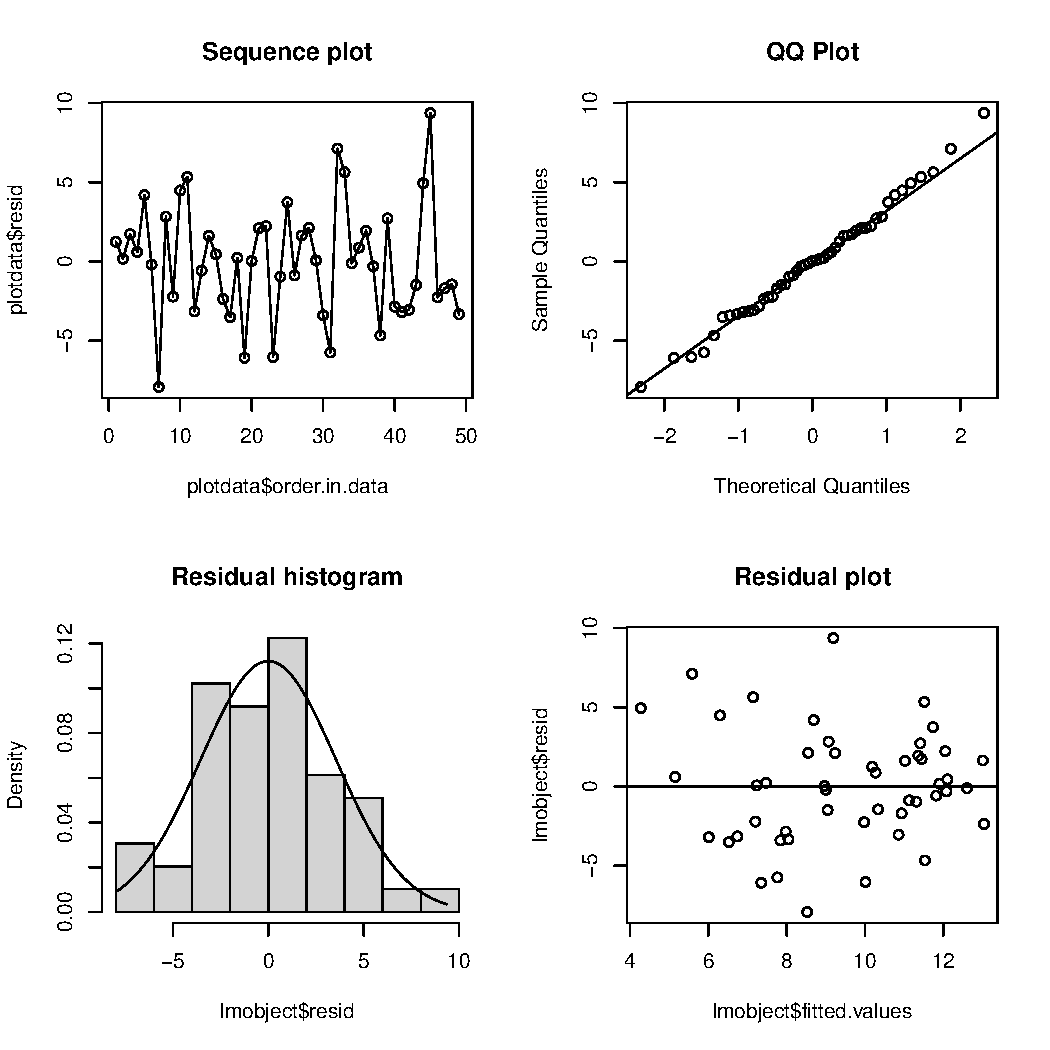
\includegraphics[width=0.6\textwidth]{figure/unnamed-chunk-8-1} 

}


\begin{kframe}\begin{alltt}
\hlstd{stat5100}\hlopt{::}\hlkwd{brown_forsythe_lm}\hlstd{(surgical_final_lm)}
\end{alltt}
\begin{verbatim}
## [1] "Brown-forsythe test for constant variance in the residuals:"
## [1] "T-statistic: 3.4794, p-value: 9e-04"
\end{verbatim}
\begin{alltt}
\hlstd{stat5100}\hlopt{::}\hlkwd{cor_normality_lm}\hlstd{(surgical_final_lm)}
\end{alltt}
\begin{verbatim}
## Correlation test of normality:
##                   resid expected_norm
## resid         1.0000000     0.9954407
## expected_norm 0.9954407     1.0000000
## 
## Total observations: 72
## Make sure to consult with table B.6 for your final result.
\end{verbatim}
\end{kframe}
\end{knitrout}

\subsubsection*{Test the trained model on the testing dataset}

\begin{knitrout}
\definecolor{shadecolor}{rgb}{0.969, 0.969, 0.969}\color{fgcolor}\begin{kframe}
\begin{alltt}
\hlstd{test_predicted} \hlkwb{<-} \hlkwd{predict}\hlstd{(surgical_final_lm,} \hlkwc{newdata} \hlstd{= test_surgical)}

\hlcom{# Get mean-squared predicted error}
\hlstd{mspr} \hlkwb{<-} \hlkwd{mean}\hlstd{((test_predicted} \hlopt{-} \hlstd{test_surgical}\hlopt{$}\hlstd{logTime)}\hlopt{^}\hlnum{2}\hlstd{)}
\hlstd{mspr}
\end{alltt}
\begin{verbatim}
## [1] 0.08472427
\end{verbatim}
\end{kframe}
\end{knitrout}

\end{document}
